\RequirePackage{plautopatch}
\RequirePackage[l2tabu, orthodox]{nag}

\documentclass[platex,dvipdfmx, a5paper]{jlreq}			% for platex
% \documentclass[uplatex,dvipdfmx]{jlreq}		% for uplatex
\usepackage{graphicx}
\usepackage[italicdiff]{physics}
\usepackage{mathtools}
\usepackage{here}
\mathtoolsset{showonlyrefs=true}
\title{生物学と力学系}

\author{木津川楓輝}
\date{}
\begin{document}
\maketitle
\thispagestyle{empty}
\section{はじめに}
最近,力学系と呼ばれる数学の手法を生物学に応用するのが流行っています.力学系は生物学のみならず,様々な分野で用いられていますが,この記事では特に細胞スケールの生物学において力学系がどのように活用されているかに焦点を当てて解説しようと思います.
\section{力学系とは}
力学系は数学の一分野なのですが,その名の通り,物理の力学をルーツとしています.物理の手法をより広い対象に適用できるようにした枠組みです.

力学系では,状態空間というものを考え,状態の時間変化を扱います.まず,状態をいくつかの変数の組で表します.変数の数を$k$として,状態を変数$\{x_1, x_2, \cdots, x_k\}$で表すと,これは$k$次元空間中の1点と見なせます.これが状態空間です.

例として,遺伝子の発現パターンを用いて細胞の状態を表すことを考えてみましょう.細胞中では,各遺伝子からmRNAが作られ,タンパク質が生成されます.それぞれのmRNAやタンパク質の量は発現量と呼ばれ,細胞状態を表す重要な指標となります.この場合,$k$個の遺伝子に注目しているとすると,各遺伝子の発現量$\{x_1, x_2, \cdots, x_k\}$が状態空間を構成します.
\section{力学系の時間発展}
ところで,一般に状態は時間とともに変化します.これは,状態空間において点が移動することに対応します.と言われてもイメージしにくいと思うので,再び遺伝子の発現パターンを例にとって説明します.今回は2つの遺伝子を考え,それらが互いに抑制しあう場合を考えることにします.具体的には,遺伝子1によって作られたタンパク質が遺伝子2の発現を抑制し,遺伝子2によって作られたタンパク質は遺伝子1の発現を抑制するといった状況です.タンパク質1, 2の濃度をそれぞれ$p_1, p_2$とすると,状態空間は $(p_1, p_2)$となります.

次に,互いに抑制する様子を式で表します.色々な場合がありますが,今回はタンパク質1, 2の単位時間あたりの合成量がそれぞれ$\frac{\alpha}{1 + p_2^2}, \frac{\alpha}{1 + p_1^2}$で表せるとします(この式はどこから出て来たんだと思われるかもしれません.ここでは述べませんが,ちゃんと化学的な理由があります).

また,タンパク質はある一定の割合で減少していきます.簡単のために,その速度定数は2つのタンパク質で共通であるとしましょう.すると,時間の単位を適当にとれば,その定数を1にすることができます.

以上をまとめると,$p_1, p_2$の時間発展を表す微分方程式は次のようになります.
\begin{align}
\dv{p_1}{t} &= \frac{\alpha}{1 + p_2^2} - p_1 \label{f1} \\
\dv{p_2}{t} &= \frac{\alpha}{1 + p_1^2} - p_2 \label{f2}
\end{align}
ところで,$\dv{p_1}{t}, \dv{p_2}{t}$は状態空間においてそれぞれ$p_1$軸,$p_2$軸方向の速度を表しています.それらが$p_1$と$p_2$によって決まっているということは,状態空間中の各点では,その点における速度の大きさと向きが決まっているということです.それを矢印の大きさと向きに対応させて上の例における状態空間を描くと,図1, 2のようになります(図が2つあるのは,パラメータ$\alpha$の値によって力学系の性質が変化するからです).
\begin{figure}[H]
 \centering
   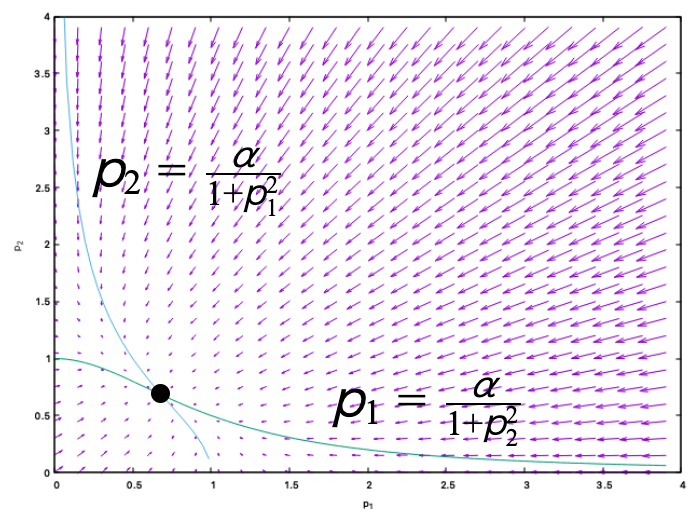
\includegraphics[width=100mm]{figures/a.png}
   \caption{ヌルクラインとフロー($\alpha < 2$)}
\end{figure}
\begin{figure}[H]
 \centering
   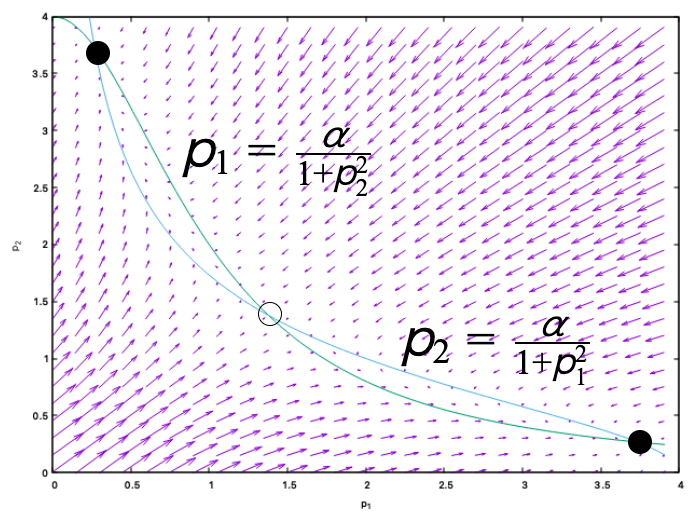
\includegraphics[width=100mm]{figures/b.png}
   \caption{ヌルクラインとフロー($\alpha > 2$)}
\end{figure}
状態空間中の点は時間とともに図中の矢印に従って流れるように移動し,それに伴って状態が変化していきます.
\section{ヌルクライン}
\eqref{f1}および\eqref{f2}の右辺が0となるような曲線のことをヌルクラインと言います.図1や図2の中にもヌルクラインが描いてあります.これがなぜ重要なのかというと,ヌルクラインを境に流れの向きが変わることが多いからです.今回の例では,\eqref{f1}の右辺が0となるヌルクラインは$p_1 = \frac{\alpha}{1 + p_2^2}$ですが,この曲線を境に\eqref{f1}の符号が変わります.$\dv{p_1}{t}$は状態空間中での$p_1$方向の速度を表していますから,このヌルクラインを境に流れの$p_1$成分の向きが変わるということになります.\eqref{f2}についても同様です.

今はコンピューターを用いて簡単に流れの状態を見ることができますが,コンピューターがまだ発達していない時代には,ヌルクラインが力学系の性質を調べるための重要な手がかりとなっていたそうです.
\section{固定点と安定性}
\eqref{f1}と\eqref{f2}の右辺が共に0となる点を固定点と言います.図中では,2本のヌルクラインの共有点が固定点です(黒や白の丸で示してあります).固定点では$p_1$方向の速度も$p_2$方向の速度も0ですから,この点で表される状態は時間が経っても変化しないということになります.ただし,全ての固定点が同じ性質を示すわけではありません.この章では固定点の安定性に着目して分類を行いたいと思います.

図1および図2の黒丸で示された固定点を見てください.分かりにくいですが,これらの固定点に向かって矢印が吸い込まれるような形になっています.つまり,これらの固定点の近くにある点は固定点に吸い込まれ,永遠に動かなくなります.このような固定点のことを安定固定点と言います.

一方,図2の白丸で示された固定点は,右上と左下からは矢印が吸い込まれているのですが,右下と左上に向かって矢印が湧き出ている形になっています.これはどういう状態かというと,ちょうどこの固定点にある状態は確かにこの状態に留まり続けるのですが,この状態から少しでも離れた場所にある点は右下または左上に流れてしまうような状態です.このような固定点のことを不安定固定点と言います.例えるなら,鉛筆の尖った方を下にして机の上に立てるようなものです.ぴったり垂直に立てることができれば理論上は鉛筆は立ち続けますが,実際には微小なずれが原因ですぐに倒れてしまいます.

このように,安定か不安定かという違いだけで固定点の性質は全く異なったものになります.実際には今回のように矢印の向きを見て調べるのではなく,計算によって厳密に解析する方法が用いられるのですが,高度なテクニックが必要になるのでここでは割愛します.

ちなみに,図2を見ていただくと,タンパク質1の濃度$p_1$が高くて(オン)タンパク質2の濃度$p_2$が低い(オフ)安定固定点と,その逆の安定固定点があることが分かります.この力学系では,どのような状態からスタートしても,時間とともに矢印に従って移動し,これらの2つの安定固定点のうち,どちらかに吸い込まれます.そのため,このような互いに抑制する遺伝子発現のシステムは,つまみでスイッチのオン・オフを切り替えるシステムにならって,トグル・スイッチと呼ばれています.
\section{終わりに}
いかがだったでしょうか.力学系は様々な対象に適用できる便利な道具ですが,今回は生物学,特に細胞スケールの現象を例にとって説明してみました.短い記事ですので生物学的な面白さにはあまり立ち入れませんでしたが,ヌルクラインや固定点の安定性といった概念は様々な現象において重要になってきます.皆さんも自分の興味がある分野で力学系が使われているかどうか,調べてみてはいかがでしょうか.最後まで読んでいただき,ありがとうございました.
\section{参考文献}
金子邦彦・澤井哲・高木拓明・古澤力『細胞の理論生物学 ダイナミクスの視点から』東京大学出版会,2020
\end{document}
